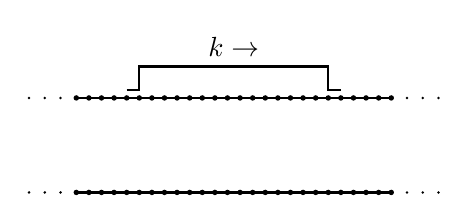
\begin{tikzpicture}[
  vert/.style={circle,fill=black,inner sep=.7pt,minimum width=0pt},
  dots/.style={circle,fill=black,inner sep=.25pt,minimum width=0pt},
  thick,
  scale=0.4]
  \foreach \x in {0,.4,...,10}{
    \node at (\x ,0) [vert]{};
    \node at (\x ,3) [vert]{};
  }

  \draw (0,0) -- (10,0);
  \draw (0,3) -- (10,3);

  \begin{scope}[yshift=0cm]
  \draw (1.6,3.25) -- (2,3.25) -- (2,4) to node [above] {$k\rightarrow$}
        (8,4) -- (8,3.25) -- (8.4,3.25);
  \end{scope}

  \foreach \xsh in {-1.5cm , 10.5cm}{
  \foreach \ysh in {0cm, 3cm}{
    \begin{scope}[xshift=\xsh,yshift=\ysh]
      \node at (0,0) [dots]{};
      \node at (0.5,0) [dots] {};
      \node at (1,0) [dots]{};
    \end{scope}
  }}
\end{tikzpicture}